\begin{anexosenv}

\partanexos

\chapter{Processo de Renderização}
\label{renderpipe}


	O processo de geração de gráficos tridimensionais em computadores tem início com a criação de cenas. Uma cena é composta por objetos, que por sua vez são compostos por primitivas geométricas (como triângulos, quadrados, linhas, entre outros) que são constituídas de vértices, estabelecendo a geometria. Todos estes vértices seguem um processo similar de processamento para formarem uma imagem na tela.  Este processo é mostrado na Figura \ref{pipeline} e as próximas seções detalham cada uma das etapas ilustradas. 

	
\section{Processamento dos Dados dos Vértices}

	A etapa de Processamento dos Dados dos Vértices é responsável por configurar os objetos utilizados para renderização com um \textit{shader} específico, dependendo da técnica de renderização de modelos tridimensionais utilizada. Uma destas técnicas é a utilização de um \textit{vertex array object}, que descreve o modelo tridimensional por meio de uma lista de vértices e uma lista de índices. Na Figura \ref{quadrado}, tem-se dois triângulos e quatro vértices definidos (dois vértices são compartilhados). Assim, pode-se definir um vetor com os vértices [v0, v1, v2, v3] e um vetor de índices [0, 3, 1, 0, 2, 3], que determina a ordem em que os vértices devem ser renderizados. 

	\begin{figure}[h]
	\centering
		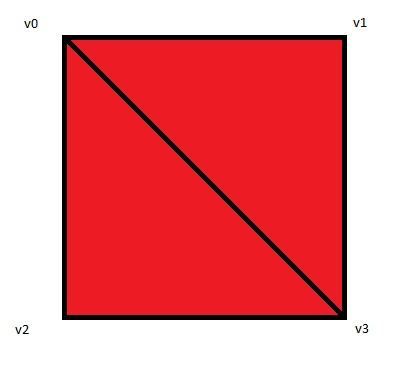
\includegraphics[keepaspectratio=true,scale=0.5]{figuras/quadrado.jpg}
	\caption{Vértices do quadrado constituído de dois triângulos}
	\label{quadrado}
	\end{figure}

	Outra técnica é a utilização de um  \textit{vertex object buffer}, em que a ideia é parecida com a da técnica anterior, porém, de acordo com \cite{vbo}, o \textit{driver} gráfico pode optar por colocar o \textit{buffer} contendo os vértices e índices diretamente na memória da GPU, melhorando o desempenho para objetos que não são modificados com muita frequência. 

\section{Processamento dos Vértices}

	É nesta etapa que modela-se parte dos efeitos visuais (a outra parte é feita durante o processamento dos fragmentos).  Estes efeitos incluem as características dos materiais atribuídos aos objetos, como também os efeitos da luz, sendo que cada efeito pode ser modelado de diferentes formas, como representações de descrições físicas. Muitos dados são armazenados em cada vértice, como a sua localização e o vetor normal associado (que indica a orientação do vértice no espaço), por exemplo. O \textit{vertex shader} é aplicado nesta etapa.

	Além disso, as transformadas são aplicadas nas coordenadas do objeto, de forma que ele possa ser posicionado, orientado e tenha um tamanho determinado. Após o ajuste das coordenadas, é dito que o objeto está localizado no espaço do mundo e, em seguida, é aplicada a transformação de visualização, que tem como objetivo estabelecer a câmera. A etapa de projeção é responsável por transformar o volume de visualização aplicando métodos de projeção, como a perspectiva e a ortográfica (também chamada de paralela). A projeção ortográfica resulta em uma caixa retangular, em que linhas paralelas permanecem paralelas após a transformação. Na perspectiva, quanto mais longe um objeto se encontra, menor ele aparecerá após a projeção: linhas paralelas tendem a convergir no horizonte. Ela resulta em um tronco de pirâmide com base retangular. 
	
\section{Pós-processamento dos Vértices}

	Durante a etapa de Pós-processamento dos Vértices, os dados da etapa anterior são guardados em \textit{buffers}. Além disso, as primitivas geradas pelas etapas anteriores poderão ser recortadas caso estejam fora do volume de visão. Ou seja, somente as primitivas gráficas que se encontram dentro do volume de visualização serão renderizadas. Assim, o recorte (chamado \textit{clipping}) é responsável por não passar adiante as primitivas que se encontram fora da visualização. Primitivas que estão parcialmente dentro são recortadas, ou seja, o vértice que está de fora não é renderizado e é substituído por um novo vértice (dentro do volume de visualização). A  Figura \ref{clip} ilustra esta ideia.

       \begin{figure}[ht]
       \centering
	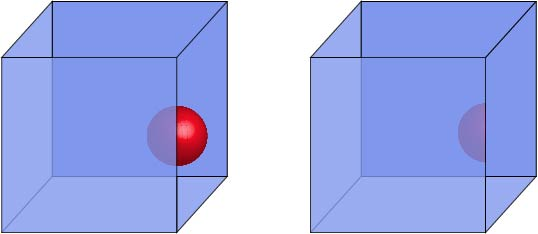
\includegraphics[keepaspectratio=true,scale=0.5]{figuras/clip.jpg}
       \caption{Antes do recorte (cubo de visualização esquerdo) e depois do recorte (cubo de visualização direito)}
       \label{clip}
       \end{figure}

\section{Montagem das Primitivas}

	A Montagem das Primitivas é o estágio em que as primitivas a serem renderizadas são enviadas. Estas primitivas são discretizadas em pontos, linhas e triângulos, em que algumas delas podem ser descartadas, baseando-se nas faces aparentes (procedimento conhecido como \textit{Face Culling}).  

\section{Conversão e Interpolação dos Parâmetros das Primitivas}

	Nesta etapa que ocorre o procedimento conhecido como rasterização. Nela, cada primitiva é transformada em fragmentos, cuja entrada é formada pelas primitivas recortadas e as coordenadas ainda tridimensionais. Assim, esta etapa tem como finalidade mapear as coordenadas tridimensionais em coordenadas de tela. Para isto, o centro de um \textit{pixel} (\textit{picture element}) é igual à coordenada 0,5. Então, \textit{pixels} de [0; 9] equivalem à cobertura das coordenadas de [0,0; 10,0). E os valores dos \textit{pixels} crescem da esquerda para a direita e de cima para baixo. Também é feita a configuração dos triângulos, em que dados são computados para as superfícies dos triângulos. Eles serão utilizados para a conversão dos dados vindos do processo de geometria (coordenadas e informações provenientes do \textit{vertex shader}) em \textit{pixels} na tela e também para o processo de interpolação. Assim, é checado se cada um dos \textit{pixels} está dentro de um triângulo ou não. Para cada \textit{pixel} que sobrepõe um triângulo, um fragmento é gerado, conforme mostrado na Figura \ref{traversal}. Cada fragmento tem informações sobre sua localização na tela, no triângulo e sua profundidade, e as propriedades dos fragmentos dos triângulos são geradas usando dados interpolados entre os três vértices do triângulo. 

  \begin{figure}[ht]
       \centering
	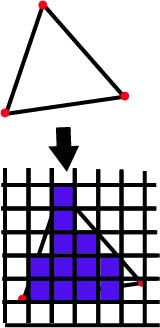
\includegraphics[keepaspectratio=true,scale=0.8]{figuras/traversal.jpg}
       \caption{Travessia de triângulos: fragmentos sendo gerados}
       \label{traversal}
       \end{figure}

\section{Processamento dos Fragmentos}

	As computações por \textit{pixel} são calculadas durante o \textit{Fragment Shading}, em que o resultado consiste em uma ou mais cores a serem passadas para o próximo estágio. Muitas técnicas podem ser aplicadas durante esta etapa, em que uma delas é a de texturização (que aplica no fragmento do objeto parte de uma imagem). 

\section{Processamento das Amostras}

	 A informação relacionada com cada \textit{pixel} é armazenada no \textit{color buffer}, que é um \textit{array} de cores. Assim, a última etapa é a de Processamento das Amostras, que realiza diversos testes nos fragmentos gerados na etapa anterior. Ela é responsável,por exemplo, pelos testes de profundidade, em que o \textit{color buffer} deve conter as cores das primitivas da cena que são visíveis do ponto de vista da câmera. Isto é feito através do Z-\textit{buffer} (também chamado de \textit{buffer} de profundidade), em que cada \textit{pixel} armazena a coordenada $z$ a partir da câmera até a primitiva mais próxima.  Então, a coordenada $z$ de uma primitiva que está sendo computada é comparada com  o valor do Z-\textit{buffer} para o mesmo \textit{pixel}. Se o valor for menor, quer dizer que a primitiva está mais próxima da câmera do que o valor da anterior, e assim, o valor do Z-\textit{buffer} é atualizado para o atual. Se o valor corrente for maior, então o valor do Z-\textit{buffer} não é modificado. Outros testes realizados são o de \textit{blending}, em que combina-se as cores do fragmento com a do \textit{buffer} e os de descarte de fragmentos, como o \textit{scissor test} e \textit{stencil test}. 	

\chapter{Representação de Objetos Tridimensionais: Formato \textit{obj}}
\label{formatobj}

	Em uma cena, os modelos tridimensionais podem variar muito mais do que formas básicas como uma esfera e um torus, por exemplo. Assim, o formato \textit{obj} foi criado pela empresa  \textit{Wavefront} e é um arquivo para leitura de objetos tridimensionais, a fim de carregar geometrias mais complexas. Segundo \cite{graphicsprog}, neste arquivo, cada linha contém informações a respeito do modelo, começando com uma palavra-chave, seguida da informação. A  Tabela \ref{palavraschave} mostra as principais palavras-chave utilizadas. 

\begin{table}[ht]
	\centering	
	\begin{tabular}{ll}
		\toprule
		\textbf{Palavra-chave} & \textbf{Significado}  \\
		\midrule
		\texttt{usemtl} & Indica se está utilizando material  \\
		\texttt{mtlib} &  Nome do material \\
		\texttt{v} &  Coordenadas x, y e z do vértice \\
		\texttt{vn} & Coordenadas da normal \\
		\texttt{vt} &  Coordenadas da textura \\
		\texttt{f} &  Face do polígono \\
		\bottomrule
	\end{tabular}
	\caption{ Palavras-chave do formato obj}
	\label{palavraschave}
\end{table}

	A face do polígono (f) possui três índices que indicam os vértices do triângulo. Assim, cada vértice possui um índice (que depende de quando ele foi declarado), começando a partir de um. O Código \ref{objFile} mostra o exemplo de um arquivo obj para a leitura de um cubo. 

	\lstinputlisting[language=Python, caption = {Representação do formato \textit{obj}}, label = {objFile}]{codigos/obj.txt}

	Então, a partir da leitura do arquivo  \textit{obj}, é possível ler cada linha e armazenar, em estruturas de dados, as informações que serão passadas para renderizar o modelo tridimensional, como vértices e índices, e utilizar um dos métodos apresentados anteriormente para renderizar a cena. 


\end{anexosenv}

